%-------------------------
% Resume in Latex
% Author : Jake Gutierrez
% Based off of: https://github.com/sb2nov/resume
% License : MIT
%------------------------

\documentclass[letterpaper,11pt]{article}

\usepackage{latexsym}
\usepackage[empty]{fullpage}
\usepackage{titlesec}
\usepackage{marvosym}
\usepackage[usenames,dvipsnames]{color}
\usepackage{verbatim}
\usepackage{enumitem}
\usepackage[hidelinks]{hyperref}
\usepackage{fancyhdr}
\usepackage[english]{babel}
\usepackage{tabularx}
\input{glyphtounicode}

%------figures

\usepackage{graphicx}
\usepackage{wrapfig}



%----------FONT OPTIONS----------
% sans-serif
% \usepackage[sfdefault]{FiraSans}
% \usepackage[sfdefault]{roboto}
% \usepackage[sfdefault]{noto-sans}
 \usepackage[default]{sourcesanspro}

% serif
% \usepackage{CormorantGaramond}
% \usepackage{charter}


\pagestyle{fancy}
\fancyhf{} % clear all header and footer fields
\fancyfoot{}
\renewcommand{\headrulewidth}{0pt}
\renewcommand{\footrulewidth}{0pt}

% Adjust margins
\addtolength{\oddsidemargin}{-0.5in}
\addtolength{\evensidemargin}{-0.5in}
\addtolength{\textwidth}{1in}
\addtolength{\topmargin}{-.5in}
\addtolength{\textheight}{1.0in}

\urlstyle{same}

\raggedbottom
\raggedright
\setlength{\tabcolsep}{0in}

% Sections formatting
\titleformat{\section}{
  \vspace{-4pt}\scshape\raggedright\large
}{}{0em}{}[\color{black}\titlerule \vspace{-5pt}]

% Ensure that generate pdf is machine readable/ATS parsable
\pdfgentounicode=1

%-------------------------
% Custom commands
\newcommand{\resumeItem}[1]{
  \item\small{
    {#1 \vspace{-2pt}}
  }
}

\newcommand{\resumeSubheading}[4]{
  \vspace{-2pt}\item
    \begin{tabular*}{0.97\textwidth}[t]{l@{\extracolsep{\fill}}r}
      \textbf{#1} & #2 \\
      \textit{\small#3} & \textit{\small #4} \\
    \end{tabular*}\vspace{-7pt}
}

\newcommand{\resumeSubSubheading}[2]{
    \item
    \begin{tabular*}{0.97\textwidth}{l@{\extracolsep{\fill}}r}
      \textit{\small#1} & \textit{\small #2} \\
    \end{tabular*}\vspace{-7pt}
}

\newcommand{\resumeProjectHeading}[2]{
    \item
    \begin{tabular*}{0.97\textwidth}{l@{\extracolsep{\fill}}r}
      \small#1 & #2 \\
    \end{tabular*}\vspace{-7pt}
}

\newcommand{\resumeSubItem}[1]{\resumeItem{#1}\vspace{-4pt}}

\renewcommand\labelitemii{$\vcenter{\hbox{\tiny$\bullet$}}$}

\newcommand{\resumeSubHeadingListStart}{\begin{itemize}[leftmargin=0.15in, label={}]}
\newcommand{\resumeSubHeadingListEnd}{\end{itemize}}
\newcommand{\resumeItemListStart}{\begin{itemize}}
\newcommand{\resumeItemListEnd}{\end{itemize}\vspace{-5pt}}

%-------------------------------------------
%%%%%%  RESUME STARTS HERE  %%%%%%%%%%%%%%%%%%%%%%%%%%%%


\begin{document}

%----------HEADING----------
% \begin{tabular*}{\textwidth}{l@{\extracolsep{\fill}}r}
%   \textbf{\href{http://sourabhbajaj.com/}{\Large Sourabh Bajaj}} & Email : \href{mailto:sourabh@sourabhbajaj.com}{sourabh@sourabhbajaj.com}\\
%   \href{http://sourabhbajaj.com/}{http://www.sourabhbajaj.com} & Mobile : +1-123-456-7890 \\
% \end{tabular*}

\begin{center}
    \textbf{\Huge \scshape Tao Sun} \\ \vspace{2pt}
    \small +86-183-0515-9970 $|$ \href{mailto:x@x.com}{\underline{s.tao@nuaa.edu.cn}} $|$ 
    \href{https://linkedin.com/in/tao-sun-431a34197}{\underline{linkedin.com/in/tao-sun-431a34197}} $|$
    \href{https://sunzhon.github.io/}{\underline{https://sunzhon.github.io/}}\\ \vspace{1.5pt}
    Address: No. 29, Yudao Street, Qinhuai District, Nanjing, Jiangsu province, China
\end{center}

%-----------Summary-----------
\section{Summary}

\begin{wrapfigure}{r}{4cm}%靠文字内容的左侧
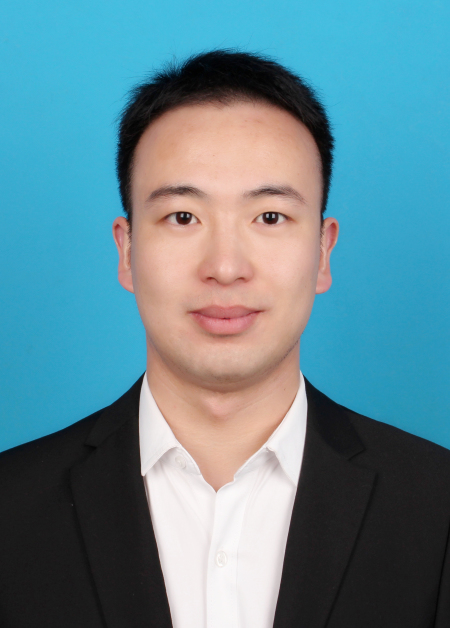
\includegraphics[width=3.4cm]{suntao.jpg}
\end{wrapfigure}Tao Sun is currently pursuing a Ph.D. degree with NEUTRON Laboratory at Nanjing University of Aeronautics and Astronautics, supervised by Prof. Poramate Manoonpong and Zhendong Dai.
His primary research aim is to investigate adaptive neural control based on central pattern generators, reflex chains, sensory feedback and learning mechanisms. The control can not only enable legged robots (e.g., quadruped robots) to autonomously generate adaptive self‐organized locomotion and also contribute to the understanding of biological neural mechanisms of animals. A secondary objective is to develop a generic adaptive neural controller, which can directly be applied in various legged robots with different morphology. The research aims have almost been accomplished. His dissertation is titled adaptive neural control for self‐organized locomotion of legged robots, and he will graduate with a PhD degree before April 2021.


%\begin{figure}
%    \centering
%    %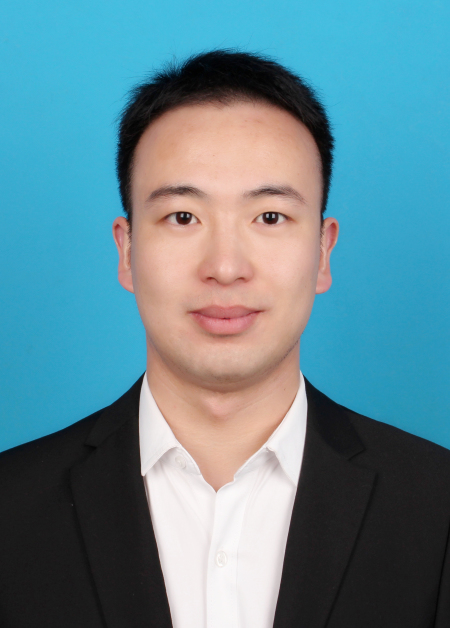
\includegraphics[width=0.5\textwidth]{suntao.jpg}
%    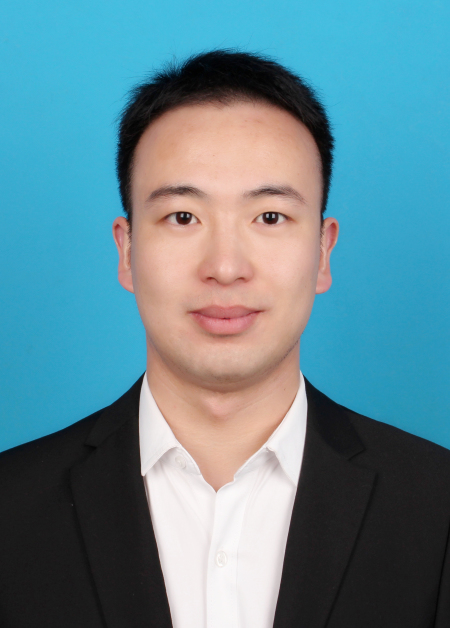
\includegraphics[width=0.2\textwidth]{suntao.jpg}
    %\caption{Caption}
    %\label{fig:my_label}
%\end{figure}

%-----------EDUCATION-----------
\section{Education}
  \resumeSubHeadingListStart
    \resumeSubheading
      {Nanjing University of Aeronautics and Astronautics}{Nanjing, China}
      {PhD of Machine design and theory}{Apr. 2016 --  Present}
    \resumeSubheading
      {Nanjing University of Aeronautics and Astronautics}{Nanjing, China}
      {Master of Machine design and theory}{Sep. 2014 -- Sep. 2016}
    \resumeSubheading
      {Anhui Polytechnic University}{Wuhu, China}
      {Bachelor of Process Equipment and Control Engineering}{Sep. 2010 -- May 2014}
  \resumeSubHeadingListEnd


%-----------EXPERIENCE-----------
\section{Experience}
\resumeSubHeadingListStart

\resumeSubheading
{PhD student}{Oct. 2020 -- Present}
{College of Mechanical and Electrical Engineering, Nanjing University of Aeronautics and Astronautics}{Nanjing, China}
\resumeItemListStart
\resumeItem{Preparing my thesis for applying a PhD degree}
\resumeItemListEnd

\resumeSubheading
{Visiting researcher}{Oct. 2019 -- Sep. 2020}
{SDU Biorobotics, University of Southern Denmark}{Odense, Denmark}
\resumeItemListStart
\resumeItem{Developed a distributed force feedback-based reflex with online learning for adaptive quadruped robot control}
\resumeItem{Performed a comparative study of adaptive interlimb coordination mechanisms for self-organized robot locomotion (comparing between continuous phase modulation and phase resetting of decoupled CPGs)}
\resumeItemListEnd

\resumeSubheading
{PhD student}{Jan. 2018 -- Sep. 2019}
{College of Mechanical and Electrical Engineering, Nanjing University of Aeronautics and Astronautics}{Nanjing, China}
\resumeItemListStart
\resumeItem{Investigated neural control with adaptive physical and neural communications for reusable quadruped locomotion}
\resumeItem{Investigated adaptive neural control for self-organized locomotion and obstacle negotiation of quadruped robots}
\resumeItem{Developed a small-sized reconfigurable quadruped robot with multiple sensory feedback}
\resumeItemListEnd

\resumeSubheading
{Robotic engineer (intern)}{Apr. 2016 -- Dec. 2017}
{The 609 Research Institute of China Aviation Industry}{Nanjing, China}
\resumeItemListStart
\resumeItem{Developed control algorithms for high slope walking of a hydraulic quadruped robot}
\resumeItem{Developed a hardware system of a hydraulic quadruped robot}
\resumeItemListEnd

\resumeSubheading
{Master student}{Jun. 2014 -- Sep. 2016}
{College of Astronautics, Nanjing University of Aeronautics and Astronautics}{Nanjing, China}
\resumeItemListStart
\resumeItem{Investigated path planning with lidar of mobile robots}
\resumeItem{Investigated gait planning and foot trajectory optimization for efficient locomotion of hydraulic quadruped robots}
\resumeItemListEnd

\resumeSubHeadingListEnd

\iffalse
%-----------PROJECTS-----------
\section{Projects}
\resumeSubHeadingListStart
\resumeProjectHeading
{\textbf{Advanced hydraulic quadruped robot} $|$ \emph{Matlab, STM32, Keil, ADAMAS, C/C++, QNX}}{Jun. 2014 -- Dec. 2017} \\ \vspace{2pt}
I participated in
\resumeItemListStart
\resumeItem{Investigated path planning based lidar of mobile robots}
\resumeItem{Investigated gait planning and foot trajectory optimization for hydraulic quadruped robots}
\resumeItem{Developed locomotion controller of hydraulic quadruped robots}
\resumeItemListEnd
\resumeProjectHeading
{\textbf{NEUTRON} $|$ \emph{Python, C/C++, Linux, ROS, CoppeliaSim, LpzRobots, Git,UG NX}}{May 2018 -- Present}
\resumeItemListStart
\resumeItem{Developed a small-sized quadruped robot with flexible configuration and multiple sensory feedback.}
\resumeItem{Investigated adaptive neural control for self-organized locomotion of quadruped robots}
\resumeItem{Investigated adaptive interlimb coordination mechanisms of self-organized quadruped locomotion}
\resumeItem{Investigated distributed GRF feedback and vestibular reflexes for stabilizing quadruped locomotion}
\resumeItemListEnd
\resumeSubHeadingListEnd

\fi


%--------------Presentation--------------------%

\section{Presentation}
\resumeSubHeadingListStart
\resumeProjectHeading 
{\textbf{Oral}}\\
\resumeItemListStart
\resumeItem{International Youth Conference of Bionic Engineering (IYCBE 2018 ), "Adaptive neural control for self-organized locomotion and obstacle negotiation of quadruped robots", 7th-9th November 2018, Odense, Denmark.}\vspace{1.5pt}
\resumeItem{China Denmark Bio-inspired Engineering Seminar, "Adaptive neural control with adaptive physical and neural communications for quadruped locomotion", 15th October 2018, Nanjing, China.}
\resumeItemListEnd

\resumeProjectHeading 
{\textbf{Post}}\\
\resumeItemListStart
\resumeItem{The 2nd National Robot Innovation and Design Competition, "A small-sized quadruped robot for studying bio-inspired locomotion control", 23rd – 26th September 2020, Xi’an, China.}\vspace{1.5pt}
\resumeItem{The 27th IEEE International Symposium on Robot and Human Interactive Communication (RO-MAN 2018), "Adaptive neural control for self-organized locomotion and obstacle negotiation of quadruped robots", Aug. 2018, Nanjing, China.}
\resumeItemListEnd
\resumeSubHeadingListEnd

%---------------Funding/Award-------------%
\section{Award}

\resumeItemListStart
\resumeItem{The third prize in the 2nd in Robot Innovation and Design Competition of China Graduate Students, 23rd – 26th September 2020, Xi’an, China.}
\resumeItem The third prize of "Jerry Cup" in Energy Equipment Innovation Design Competition of China Graduate Students, 2020, China.
\resumeItem{Scholarship for supporting visiting research  one year in Denmark from China Scholarship Council, 2019, China}
\resumeItem{The third prize in the 7th “Tiangong Cup” of postgraduate innovative experiment competition, 30th November 2018, China.}
\resumeItemListEnd


%------------------Publication----------------
\section{Publications}

\begin{enumerate}
\item \textbf{Sun, T.}, Shao, D., Dai, Z., \& Manoonpong, P. (2018, August). Adaptive neural control for self-organized locomotion and obstacle negotiation of quadruped robots. In 2018 27th IEEE International Symposium on Robot and Human Interactive Communication (RO-MAN) (pp. 1081-1086). IEEE.
\item \textbf{Sun, T.}, Xiong, X., Dai, Z., \& Manoonpong, P. (2020). Small-Sized Reconfigurable Quadruped Robot With Multiple Sensory Feedback for Studying Adaptive and Versatile Behaviors. Frontiers in Neurorobotics, 14, 14.
\item \textbf{Sun, T.}, Dai, Z., \& Manoonpong, P. (2020.1). Robust and reusable self-organized locomotion of legged robots under adaptive physical and neural communications. IEEE Transactions on Cybernetics (revision).
\item \textbf{Sun, T.}, Dai, Z., \& Manoonpong, P. (2020.8). Distributed-force-feedback-based reflex with online learning for adaptive quadruped motor control. Neural Networks (Accepted).
\item \textbf{Sun, T.}, Xiong, X., Dai, Z., Dai O., \& Manoonpong, P. (2020). A comparative study of adaptive interlimb coordination mechanisms for self-organized robot locomotion. Frontiers in robotics and AI.
\item Mario Calandra, Luca Patane, \textbf{Tao Sun}, Paolo Arena, Manoonpong P. (2020). Echo State Networks for estimating exteroceptive conditions from proprioceptive states in quadruped robots. Frontiers in Neurorobotics (under review)
\end{enumerate}

%-------------------Teaching-----------------
\section{Teaching}
\begin{enumerate}
    \item Teaching "Phase adaptation under physical and neural communication for stable self-organized locomotion" in Embodied AI and Robotics Course, University of Southern Denmark, Nov. 7th 2019.
    \item Teaching "Decoupled CPGs-based control for self-organized locomotion of legged robot” in  Adaptive Locomotion Control Course, Nanjing University of Aeronautics and Astronautics, Dec. 5th  2020.
\end{enumerate}



%-----------PROGRAMMING SKILLS-----------
\section{Technical Skills}
\begin{itemize}[leftmargin=0.15in, label={}]
\small{\item{
\textbf{Languages}{: Matlab, Python, C/C++, Lua, Latex} \\
\textbf{Platforms}{: Ubuntu, ADAMAS, ROS, CoppeliaSim, LpzRobots, Webots} \\
\textbf{Developer Tools}{: Git, Eclipse, Vim, UG NX, Inkscape, Kdenlive} \\
%\textbf{Libraries}{: pandas, NumPy, Matplotlib}
}}
\end{itemize}


%--------------------Referees--------------------%

\iffalse

\section{Referees}
\resumeItemListStart

\resumeItem{Professor Poramate Manoonpong, Embodied AI \& Neurobotics Lab, SDU Biorobotics, the Mærsk Mc-Kinney Møller Institute, the University of Southern Denmark, Odense M, Denmark\\
Email:\href{mailto:x@x.com}{ \underline{poma@mmmi.sdu.dk}} Phone: +45 65508698}\\

\resumeItem{Professor Zhendong Dai, the institute of Bio‑inspired Structure and Surface
Engineering, College of Mechanical and Electrical Engineering, Nanjing Univeristy of Aeronautics and Astronautics, Nanjing, China\\
Email:\href{mailto:x@x.com}{ \underline{zddai@nuaa.edu.cn}} Phone: +45 13851810563}

\resumeItemListEnd

\fi
\end{document}
